\documentclass[11pt]{article}

\pdfobjcompresslevel=3    % compress PDF objects
\pdfcompresslevel=9       % compress streams more (0..9)
\pdfminorversion=4

\usepackage[utf8]{inputenc} % remove if using XeLaTeX or LuaLaTeX
\usepackage[T1]{fontenc}
\usepackage{polski}[babel]

% Layout & graphics
\usepackage[a4paper, total={7.5in, 9in}]{geometry}
\usepackage{graphicx}
\usepackage{wrapfig}              % images
\usepackage[dvipsnames,table]{xcolor} % single xcolor invocation (keeps table option)

% Math & symbols
\usepackage{amsmath}
\usepackage{amssymb}
\usepackage{gensymb}

% Typography & layout helpers
\usepackage{microtype}
\usepackage{float}                 % [H] placement
\usepackage{caption}
\usepackage{subcaption}            % modern subfigure support (do NOT load subfig)
\usepackage{multirow}
\usepackage{titlesec}

\usepackage{lmodern}
\usepackage{listings}
\usepackage{xcolor}

\geometry{margin=2.5cm}

% Kolory dla listingow kodu
\definecolor{codegreen}{rgb}{0,0.6,0}
\definecolor{codegray}{rgb}{0.5,0.5,0.5}
\definecolor{codepurple}{rgb}{0.58,0,0.82}
\definecolor{backcolour}{rgb}{0.95,0.95,0.92}
\definecolor{codeblue}{rgb}{0,0,0.7}

\definecolor{xppblue}{RGB}{37, 150, 190}

% Styl dla kodu C
\lstdefinestyle{cstyle}{
    backgroundcolor=\color{backcolour},   
    commentstyle=\color{codegreen},
    keywordstyle=\color{codeblue}\bfseries,
    numberstyle=\tiny\color{codegray},
    stringstyle=\color{codepurple},
    basicstyle=\ttfamily\footnotesize,
    breakatwhitespace=false,         
    breaklines=true,                 
    captionpos=b,                    
    keepspaces=true,                 
    numbers=left,                    
    numbersep=5pt,                  
    showspaces=false,                
    showstringspaces=false,
    showtabs=false,                  
    tabsize=2,
    language=C,
    frame=single,
    rulecolor=\color{codegray},
    literate={ą}{{\k{a}}}1 {ć}{{\'c}}1 {ę}{{\k{e}}}1 {ł}{{\l{}}}1 {ń}{{\'n}}1 {ó}{{\'o}}1 {ś}{{\'s}}1 {ź}{{\'z}}1 {ż}{{\.z}}1
             {Ą}{{\k{A}}}1 {Ć}{{\'C}}1 {Ę}{{\k{E}}}1 {Ł}{{\L{}}}1 {Ń}{{\'N}}1 {Ó}{{\'O}}1 {Ś}{{\'S}}1 {Ź}{{\'Z}}1 {Ż}{{\.Z}}1
}

% Styl dla kodu Python
\lstdefinestyle{pythonstyle}{
    backgroundcolor=\color{backcolour},   
    commentstyle=\color{codegreen},
    keywordstyle=\color{codeblue}\bfseries,
    numberstyle=\tiny\color{codegray},
    stringstyle=\color{codepurple},
    basicstyle=\ttfamily\footnotesize,
    breakatwhitespace=false,         
    breaklines=true,                 
    captionpos=b,                    
    keepspaces=true,                 
    numbers=left,                    
    numbersep=5pt,                  
    showspaces=false,                
    showstringspaces=false,
    showtabs=false,                  
    tabsize=2,
    language=Python,
    frame=single,
    rulecolor=\color{codegray},
    literate={ą}{{\k{a}}}1 {ć}{{\'c}}1 {ę}{{\k{e}}}1 {ł}{{\l{}}}1 {ń}{{\'n}}1 {ó}{{\'o}}1 {ś}{{\'s}}1 {ź}{{\'z}}1 {ż}{{\.z}}1
             {Ą}{{\k{A}}}1 {Ć}{{\'C}}1 {Ę}{{\k{E}}}1 {Ł}{{\L{}}}1 {Ń}{{\'N}}1 {Ó}{{\'O}}1 {Ś}{{\'S}}1 {Ź}{{\'Z}}1 {Ż}{{\.Z}}1
}

\lstset{style=cstyle}

\begin{document}

\begin
{table}[H]
\centering
\begin
{tabular}{|p{4cm}|p{8cm}|p{2cm}|}
\hline
\multicolumn{2}{|c|}{\cellcolor{xppblue}\textcolor[rgb]{1,1,1}{Politechnika Poznańska}}  & \multicolumn{1}{c|}{\multirow{3}{*}{\resizebox{14mm}{!}{
\includegraphics{img/logo2.eps}}}}\\
\multicolumn{2}{|c|}{\cellcolor{xppblue}\textcolor[rgb]{1,1,1}{Wydział Automatyki, Robotyki i Elektrotechniki}} & \\
\multicolumn{2}{|c|}{\cellcolor{xppblue}\textcolor[rgb]{1,1,1}{Instytut Robotyki i Inteligencji Maszynowej}} & \\
\hline
\multicolumn{1}{|c|}{AiR Sem 5} & \multicolumn{1}{c|}{Systemy mikroprocesorowe} & \multicolumn{1}{c|}{2025/26 (s.zim.)} \\
\hline
Jan Andrzejewski \par Matuesz Banaszak \par Piotr Bednarek & \textbf{Raport z projektu zaliczeniowego} \par Balansująca piłka na pochylni & Data wyk.:\par 13.10.20\\
\hline
Grupa środa 13:30  & &  \\
\hline
\end{tabular}
\end{table}

\tableofcontents
\newpage

\section{Wprowadzenie}

TODO tutaj jakis tekst opis celu projektu i jakies innne pierdoly

\begin{figure}[H]
    \centering
    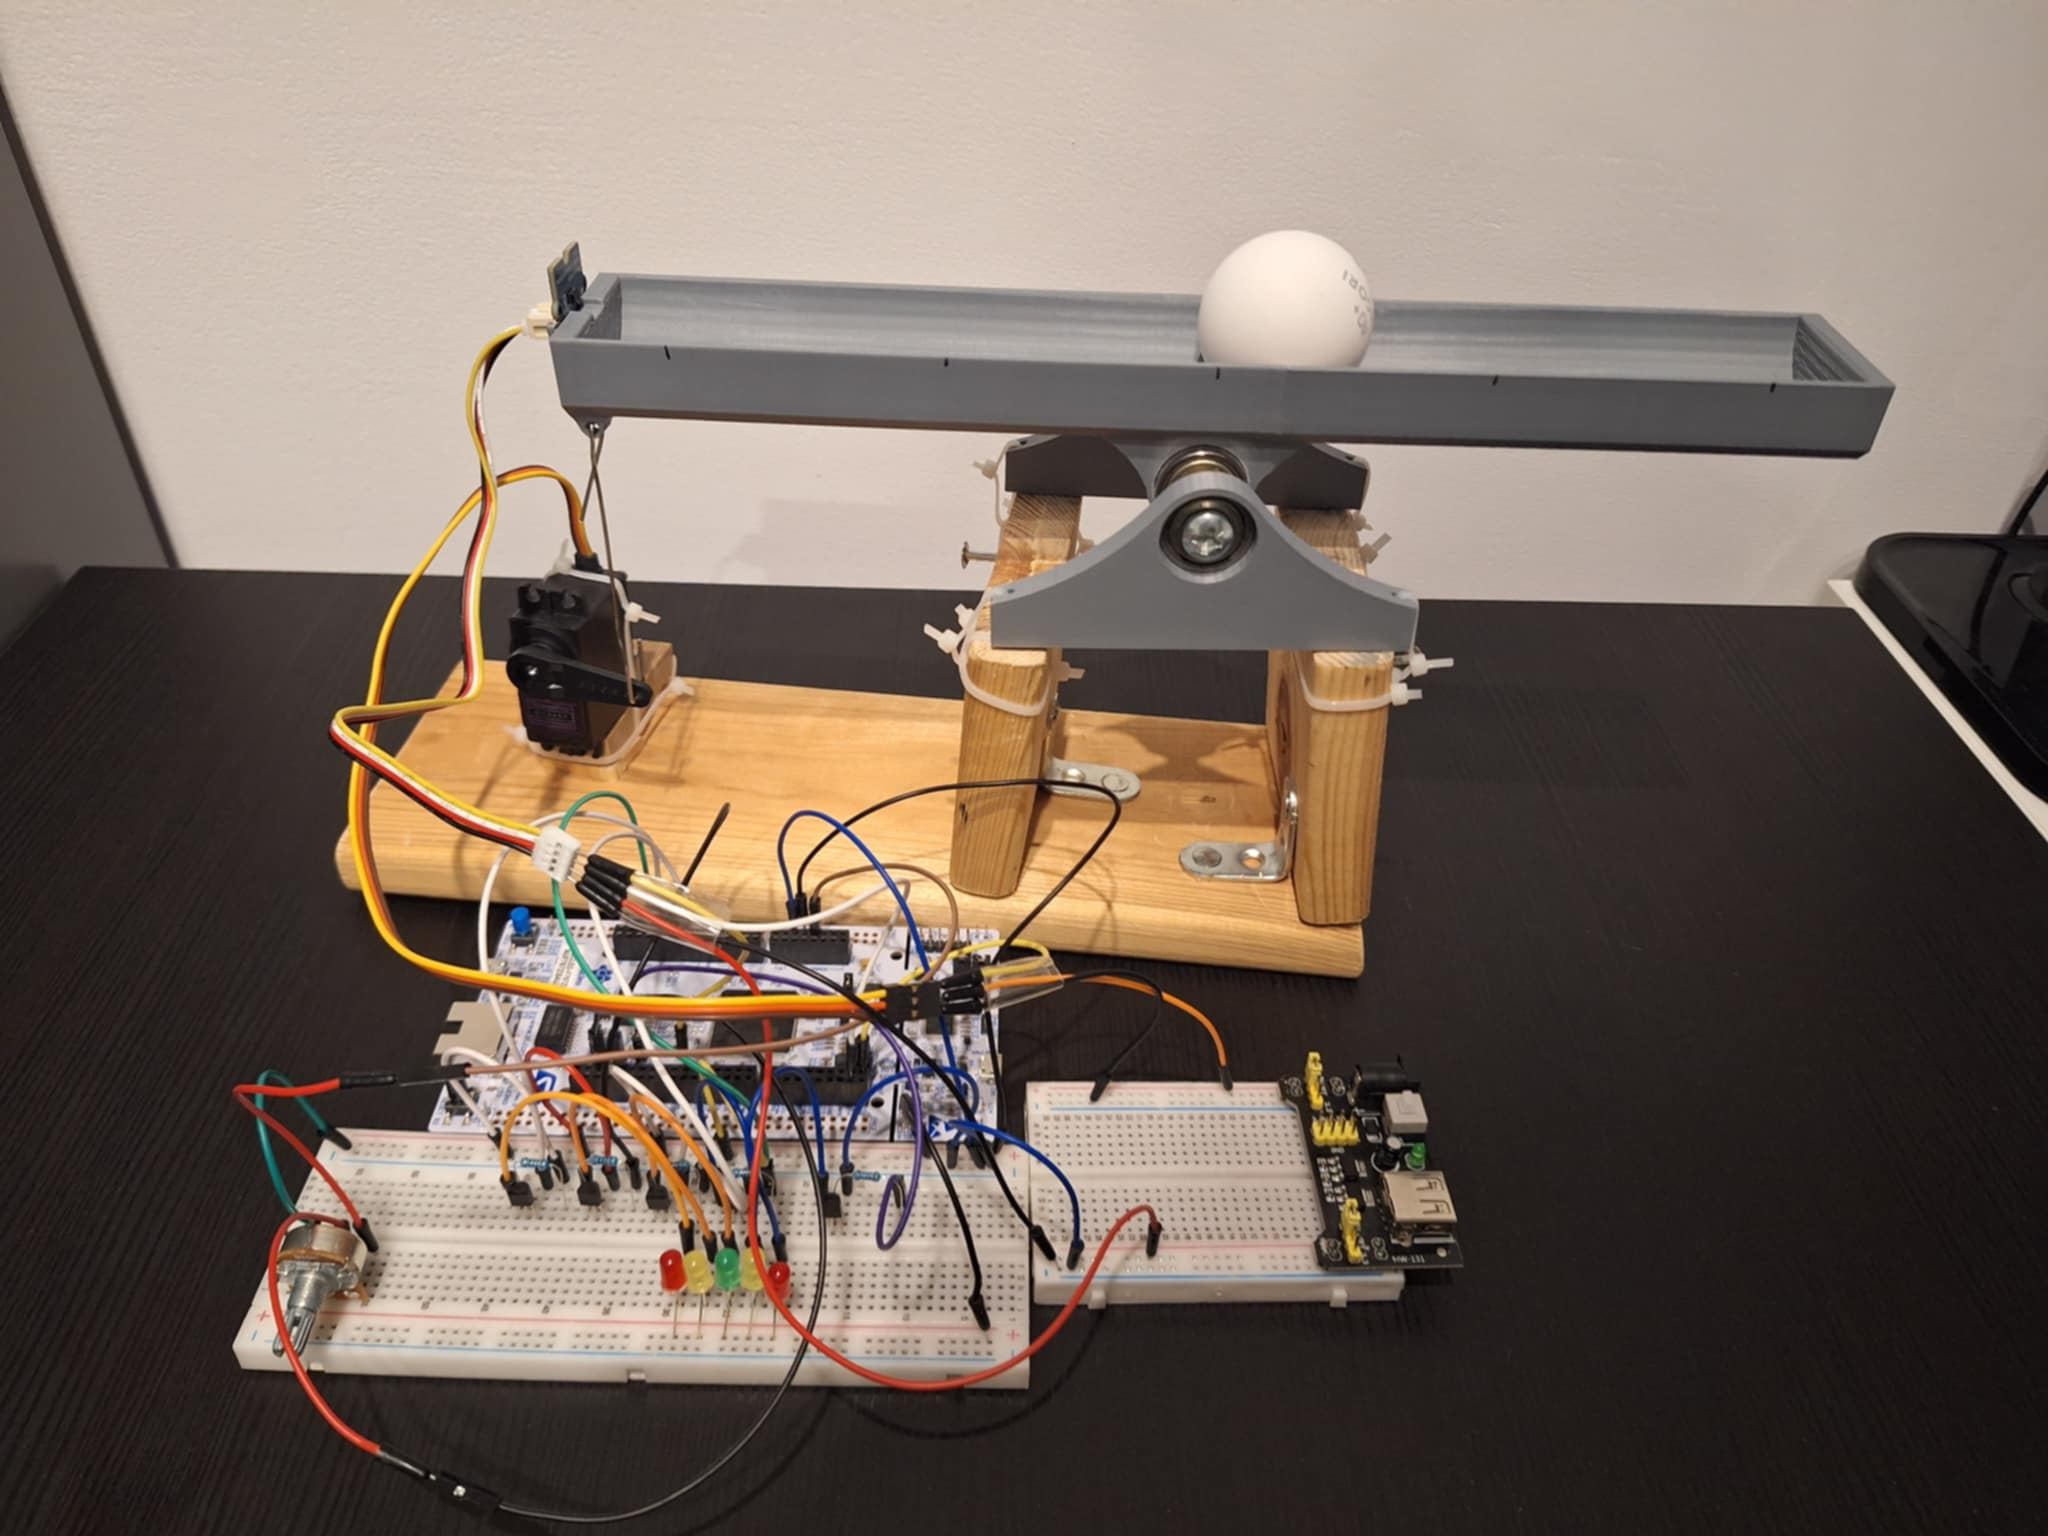
\includegraphics[width=0.7\linewidth]{img/stanowisko.png}
    \caption{Stanowisko}
\end{figure}

\begin{figure}[H]
    \centering
    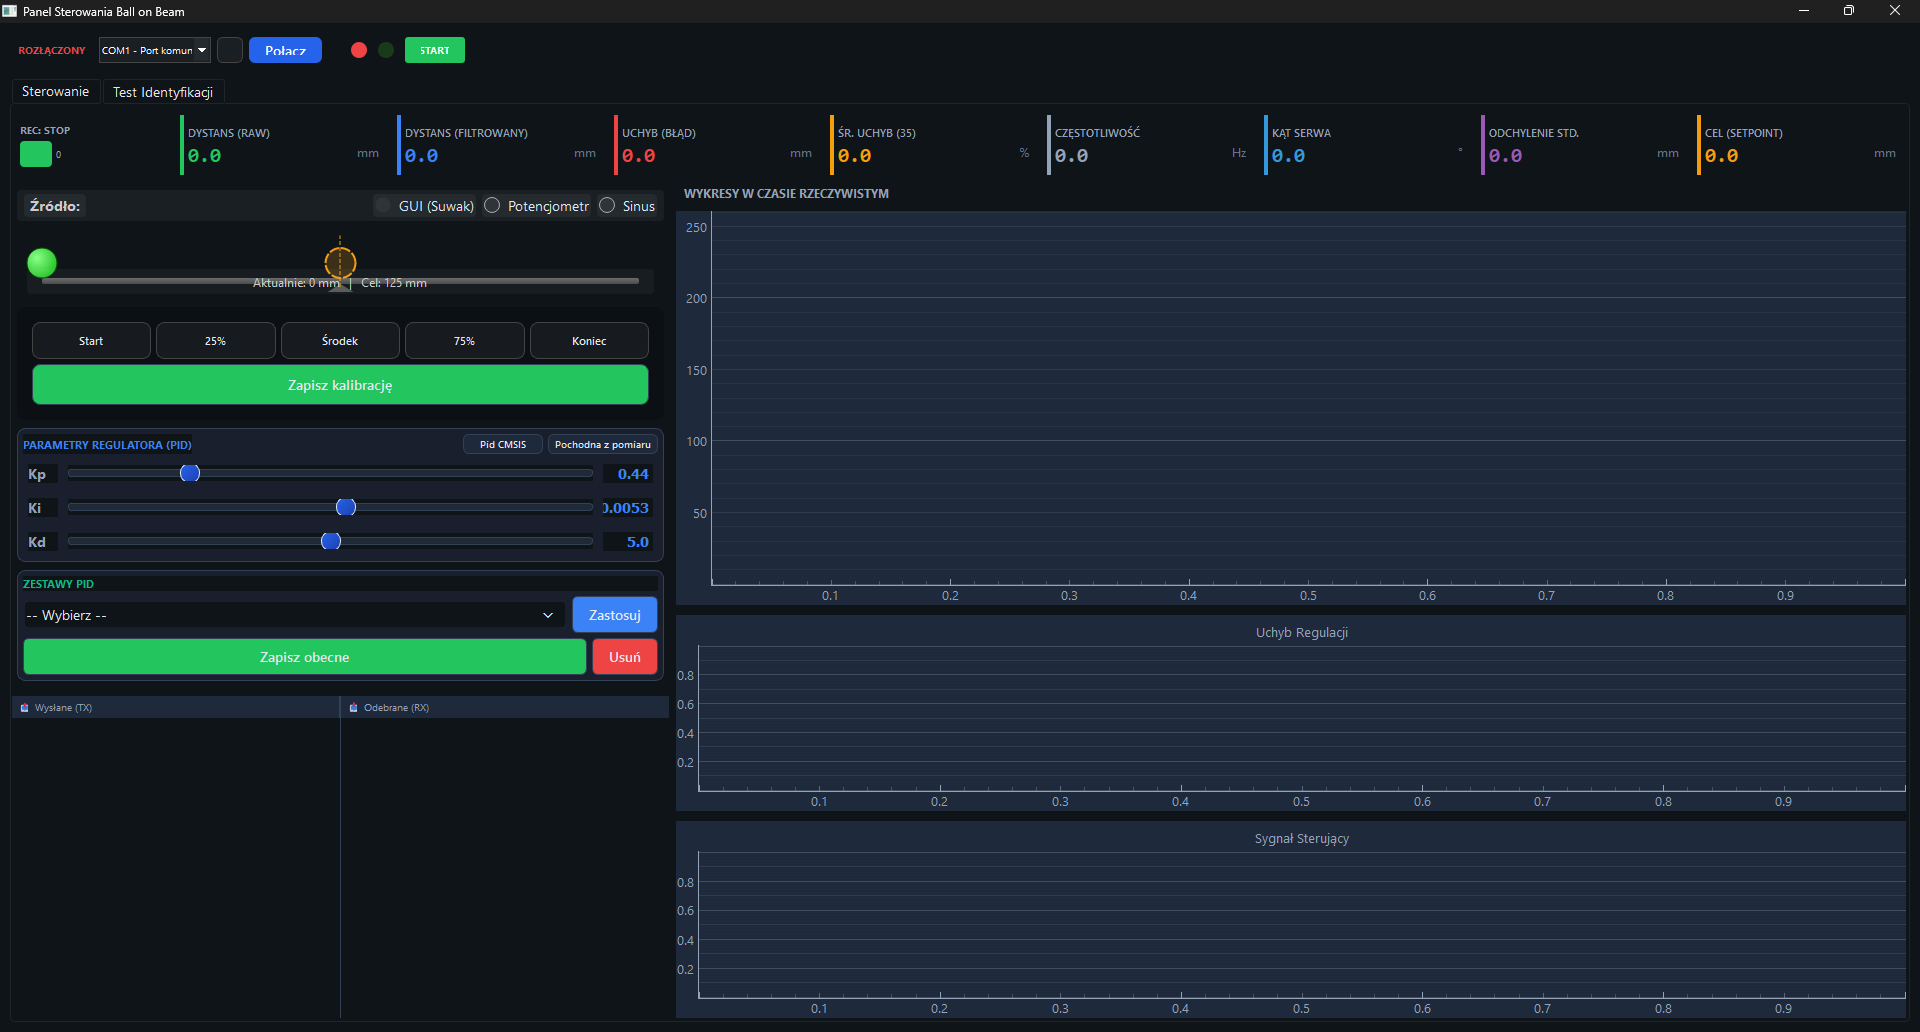
\includegraphics[width=0.7\linewidth]{img/desktop.png}
    \caption{Aplikacja desktopowa}
\end{figure}


%%%%%%%%%%%%%%%%%%%%%%%%%%%%%%%%%%%%%%%%%%%%%%%%%%%%%%%%%%%%%%%%%%%%%%%%%%%%%%%
\section{Wymagania projektowe}
%%%%%%%%%%%%%%%%%%%%%%%%%%%%%%%%%%%%%%%%%%%%%%%%%%%%%%%%%%%%%%%%%%%%%%%%%%%%%%%

Ponizej przedstawiono wymagania projektowe wraz z fragmentami kodu zrodlowego, ktore potwierdzaja ich spelnienie.

%------------------------------------------------------------------------------
\subsection{Pomiar zmiennej regulowanej ze stalym okresem probkowania}
%------------------------------------------------------------------------------

System dokonuje pomiaru regulowanej zmiennej (pozycji kulki) ze stalym okresem probkowania zdefiniowanym jako \texttt{PID\_DT\_MS = 30ms}. Zapewnia to funkcja \texttt{osDelay()} systemu FreeRTOS wywolana na koncu petli sterowania.

\begin{lstlisting}[caption={Staly okres probkowania (main.h)}, style=cstyle]
// --- Global System Settings ---
#define PID_DT_MS          30
#define SETPOINT_DEFAULT   125.0f
#define BALL_RADIUS        20
#define AVG_ERR_SAMPLES    35
\end{lstlisting}

\begin{lstlisting}[caption={Implementacja stalego okresu w petli sterowania (main.c)}, style=cstyle]
/* Infinite loop */
for (;;) {
    loop_counter++;
    
    // ... kod sterowania ...
    
    // Odczyt dystansu w trybie continuous
    distance = readRangeContinuousMillimeters(&distanceStr);
    
    // ... obliczenia PID ...
    
    osDelay(PID_DT_MS); // Loop delay - staly okres 30ms
}
\end{lstlisting}

%------------------------------------------------------------------------------
\subsection{Sterowanie w bezpiecznym zakresie zmian regulowanej zmiennej}
%------------------------------------------------------------------------------

System zapewnia bezpieczne sterowanie poprzez zdefiniowanie twardych limitow kata serwa w pliku \texttt{main.h} oraz ich egzekwowanie w kodzie sterowania.

\begin{lstlisting}[caption={Definicje limitow bezpieczenstwa serwa (main.h)}, style=cstyle]
// --- Servo Configuration ---
#define SERVO_CENTER       100.0f
#define SERVO_MIN_LIMIT    60.0f
#define SERVO_MAX_LIMIT    140.0f
#define SERVO_ANGLE_DEADBAND 0.8f
\end{lstlisting}

\begin{lstlisting}[caption={Saturacja wyjscia PID (main.c)}, style=cstyle]
// Zabezpieczenie przed NaN (Not a Number)
if (isnan(pid_angle) || isinf(pid_angle)) {
    pid_angle = SERVO_CENTER;
}

if (pid_angle < SERVO_MIN_LIMIT)
    pid_angle = SERVO_MIN_LIMIT;
else if (pid_angle > SERVO_MAX_LIMIT)
    pid_angle = SERVO_MAX_LIMIT;

// Bezposrednie sterowanie serwem
volatile float smoothed_angle = pid_angle;
SetServoAngle(smoothed_angle);
\end{lstlisting}

%------------------------------------------------------------------------------
\subsection{Uchyb ustalony na poziomie 5\% (i 1\%) zakresu regulacji}
%------------------------------------------------------------------------------

System oblicza sredni blad (rolling average) z ostatnich 35 probek, co pozwala na monitorowanie uchybu ustalonego. Zakres regulacji wynosi 250mm, wiec 5\% = 12.5mm, a 1\% = 2.5mm.

Wartosc sredniego uchybu jest przesylana przez UART i wyswietlana w czasie rzeczywistym w aplikacji desktopowej na panelu metryk oraz na wykresie. Umozliwia to biezaca ocene jakosci regulacji bez koniecznosci analizy surowych danych.

%------------------------------------------------------------------------------
\subsection{Zadawanie wartosci referencyjnej za pomoca komunikacji szeregowej lub urzadzenia wejscia}
%------------------------------------------------------------------------------

Wartosc referencyjna moze byc zadawana na dwa sposoby:
\begin{itemize}
    \item Przez komunikacje szeregowa UART (komenda \texttt{S:wartosc})
    \item Przez potencjometr podlaczony do wejscia ADC (PA0)
\end{itemize}

\begin{lstlisting}[caption={Obsluga komendy setpointu przez UART (main.c)}, style=cstyle]
void StartDefaultTask(void const * argument) {
    for (;;) {
        // Obsluga komend UART
        if (cmd_received) {
            if (rx_buffer[0] == 'S' && rx_buffer[1] == ':') {
                g_setpoint = atof((char*) &rx_buffer[2]); // S:Setpoint
                if (g_setpoint < 0.0f)
                    g_setpoint = 0.0f;
                if (g_setpoint > 250.0f)
                    g_setpoint = 250.0f;
            }
            // ... inne komendy ...
            cmd_received = 0;
        }
        osDelay(5);
    }
}
\end{lstlisting}

\begin{lstlisting}[caption={Odczyt setpointu z potencjometru ADC (main.c)}, style=cstyle]
// --- Obsluga Potencjometru ---
HAL_ADC_Start(&hadc1);
if (HAL_ADC_PollForConversion(&hadc1, 10) == HAL_OK) {
    g_adc_raw = HAL_ADC_GetValue(&hadc1);
    float pot_setpoint = (float)g_adc_raw * 0.070818f; 
    g_pot_setpoint = pot_setpoint; 
    
    // Jesli tryb Analog, nadpisz setpoint
    if (control_mode == 1) {
        // Lekki filtr na setpoint z potencjometru
        static float pot_ema = 0.0f;
        if (pot_ema == 0.0f) pot_ema = pot_setpoint;
        pot_ema = 0.1f * pot_setpoint + 0.9f * pot_ema;
        g_setpoint = pot_ema;
    }
}
HAL_ADC_Stop(&hadc1);
\end{lstlisting}

%------------------------------------------------------------------------------
\subsection{Podglad sygnalow przez komunikacje szeregowa}
%------------------------------------------------------------------------------

System wysyla dane pomiarowe przez UART w formacie tekstowym z suma kontrolna CRC-8. Dane zawieraja: dystans surowy (D), setpoint (Z), kat serwa (A), dystans filtrowany (F), blad (E), sredni blad (V) oraz status sensora (S).

\begin{lstlisting}[caption={Wysylanie danych przez UART z CRC (main.c)}, style=cstyle]
char data_buffer[64];
// D:Dist (raw); A:Angle; F:Filtered; E:Error; V:AvgError; S:Status; Z:Setpoint
int len = sprintf(data_buffer, "D:%d;Z:%d;A:%d;F:%d;E:%d;V:%d;S:%d", 
    (int)raw_distance, (int)g_setpoint, (int)smoothed_angle, 
    (int)filtered_dist, (int)current_error, (int)avg_error, 
    distanceStr.rangeStatus);

uint8_t out_crc = CalculateCRC8(data_buffer, len);

sprintf(msg, "%s;C:%02X\r\n", data_buffer, out_crc);
static uint8_t u_throttle = 0;
if (++u_throttle >= 2) {
    u_throttle = 0;
    HAL_UART_Transmit(&huart3, (uint8_t*) msg, strlen(msg), 10);
}
\end{lstlisting}

%------------------------------------------------------------------------------
\subsection{Podzial kodu na moduly i dokumentacja Doxygen}
%------------------------------------------------------------------------------

Kod zrodlowy jest podzielony na osobne moduly o jasno zdefiniowanych funkcjonalnosciach. Kazdy modul posiada dokumentacje zgodna ze standardem Doxygen.

\textbf{Struktura modulow STM32:}
\begin{itemize}
    \item \texttt{main.c/h} -- glowna aplikacja, konfiguracja peryferiow
    \item \texttt{pid.c/h} -- wrapper na CMSIS DSP PID
    \item \texttt{servo\_pid.c/h} -- wlasna implementacja PID z Anti-Windup
    \item \texttt{filters.c/h} -- filtry cyfrowe (Mediana, EMA, 1-Euro)
    \item \texttt{crc8.c/h} -- obliczanie sumy kontrolnej CRC-8
    \item \texttt{leds.c/h} -- wizualizacja bledu na LEDach
    \item \texttt{calibration.c/h} -- kalibracja sensora
\end{itemize}

\begin{lstlisting}[caption={Przyklad dokumentacji Doxygen (pid.c)}, style=cstyle]
/**
 ******************************************************************************
 * @file    pid.c
 * @author  Piotr Bednarek Jan Andrzejewski Mateusz Banaszak
 * @date    Jan 8, 2026
 * @brief   Wrapper na biblioteke CMSIS DSP PID.
 *
 * Plik zawiera funkcje inicjalizujace i obslugujace regulator PID
 * z wykorzystaniem zoptymalizowanej biblioteki matematycznej ARM (CMSIS DSP).
 ******************************************************************************
 */

/**
 * @brief Inicjalizuje regulator PID.
 *        Ustawia wspolczynniki wzmocnienia oraz limity wyjscia (nasycenie).
 *        Wywoluje arm_pid_init_f32 aby zresetowac stan wewnetrzny algorytmu.
 * @param pid Wskaznik do struktury PID_Controller_t.
 * @param Kp Wzmocnienie proporcjonalne.
 * @param Ki Wzmocnienie calkujace.
 * @param Kd Wzmocnienie rozniczkujace.
 * @param min_out Dolny limit wyjscia.
 * @param max_out Gorny limit wyjscia.
 */
void PID_Init(PID_Controller_t *pid, float Kp, float Ki, float Kd, 
              float min_out, float max_out) {
    // ...
}
\end{lstlisting}

%------------------------------------------------------------------------------
\subsection{Wykorzystanie systemu kontroli wersji}
%------------------------------------------------------------------------------

Projekt wykorzystuje system kontroli wersji Git. Repozytorium znajduje sie w katalogu glownym projektu (\texttt{.git/}).

\begin{figure}[H]
    \centering
    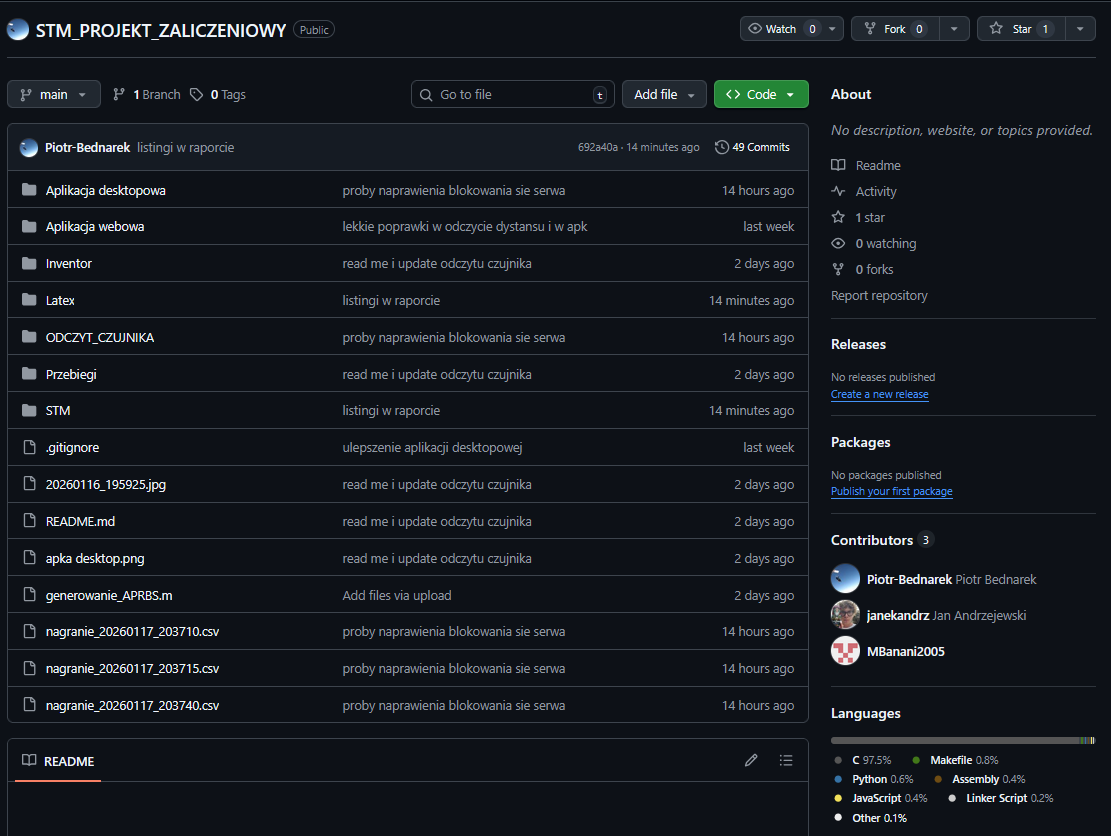
\includegraphics[width=0.7\linewidth]{img/repogithub.png}
    \caption{}
\end{figure}



%------------------------------------------------------------------------------
\subsection{Dedykowana aplikacja desktopowa (GUI)}
%------------------------------------------------------------------------------

Aplikacja desktopowa zostala napisana w jezyku Python z wykorzystaniem frameworka PySide6 (Qt). Umozliwia ona:
\begin{itemize}
    \item Polaczenie z mikrokontrollerem przez port szeregowy
    \item Wizualizacje sygnalow w czasie rzeczywistym (wykresy PyQtGraph)
    \item Zadawanie wartosci referencyjnej i parametrow PID
    \item Nagrywanie i eksport danych do CSV
    \item Sterowanie trybem pracy regulatora (Start/Stop)
\end{itemize}

\begin{lstlisting}[caption={Glowna klasa aplikacji GUI (app.py)}, style=pythonstyle]
from PySide6.QtWidgets import QMainWindow, QWidget, QVBoxLayout, QHBoxLayout
from serial_manager import SerialManager
from widgets.metrics_panel import MetricsPanel
from widgets.control_panel import ControlPanel
from widgets.charts_panel import ChartsPanel
from widgets.terminal import Terminal

class MainWindow(QMainWindow):
    def __init__(self):
        super().__init__()
        
        self.setWindowTitle("Panel Sterowania Ball on Beam")
        self.resize(1280, 800)
        
        # --- Managers ---
        self.serial = SerialManager()
        self.data_history = []
        
        # --- Recording State ---
        self.is_recording = False
        self.recording_data = []
        
        # ... konfiguracja UI ...
\end{lstlisting}

\begin{lstlisting}[caption={Manager komunikacji szeregowej (serial\_manager.py)}, style=pythonstyle]
class SerialManager(QObject):
    """
    High-level manager for Serial communication. 
    Handles Thread management, Parsing, and Signal emission.
    """
    # Signals for UI
    connected = Signal(bool)
    rx_log = Signal(str, str)  # msg, type (info/error/success)
    tx_log = Signal(str)
    new_data = Signal(dict)    # Parsed data object
    ports_listed = Signal(list)
    
    def send_setpoint(self, val):
        self.send_command(f"S:{val:.1f}")
        
    def send_pid(self, kp, ki, kd):
        self.send_pid_p(kp)
        QThread.msleep(500)
        self.send_pid_i(ki)
        QThread.msleep(500)
        self.send_pid_d(kd)
\end{lstlisting}

%------------------------------------------------------------------------------
\subsection{Skrypty do logowania sygnalow}
%------------------------------------------------------------------------------

Aplikacja desktopowa posiada wbudowany mechanizm nagrywania danych pomiarowych do plikow CSV z mozliwoscia eksportu.

\begin{lstlisting}[caption={Funkcja zapisu nagrania do CSV (app.py)}, style=pythonstyle]
def _save_recording(self):
    # Generate default filename with timestamp
    timestamp = datetime.now().strftime("%Y%m%d_%H%M%S")
    default_filename = f"nagranie_{timestamp}.csv"
    
    # Open file dialog
    filepath, _ = QFileDialog.getSaveFileName(
        self,
        "Zapisz nagranie",
        default_filename,
        "CSV Files (*.csv);;All Files (*)"
    )
    
    if filepath:
        try:
            with open(filepath, 'w', newline='', encoding='utf-8') as f:
                fieldnames = ['time', 'distance', 'filtered', 
                              'setpoint', 'error', 'control']
                writer = csv.DictWriter(f, fieldnames=fieldnames)
                writer.writeheader()
                writer.writerows(self.recording_data)
        except Exception as e:
            self.terminal.append_rx(f"Blad zapisu: {e}", "error")
\end{lstlisting}

%------------------------------------------------------------------------------
\subsection{Dodatkowe urzadzenie wyjscia -- wyswietlacz LED}
%------------------------------------------------------------------------------

System posiada 5 diod LED (PE2--PE6) wizualizujacych aktualny uchyb regulacji:
\begin{itemize}
    \item LED zielona (PE4) -- blad w zakresie $\pm$1\% (2.5mm)
    \item LEDy zolte (PE3, PE5) -- blad w zakresie $\pm$5\% (12.5mm)
    \item LEDy czerwone (PE2, PE6) -- blad wiekszy niz 5\%
\end{itemize}

\begin{lstlisting}[caption={Definicje pinow LED (main.h)}, style=cstyle]
// --- LED Error Bar ---
#define LED_ERR_PORT      GPIOE
#define LED_ERR_1_Pin     GPIO_PIN_2
#define LED_ERR_2_Pin     GPIO_PIN_3
#define LED_ERR_3_Pin     GPIO_PIN_4
#define LED_ERR_4_Pin     GPIO_PIN_5
#define LED_ERR_5_Pin     GPIO_PIN_6
\end{lstlisting}

\begin{lstlisting}[caption={Update stanu ledów (leds.c)}, style=cstyle]
void UpdateErrorLEDs_5LED(float error) {
	// Wyłącz wszystkie LEDy (PE2..PE6)
	HAL_GPIO_WritePin(GPIOE, LED_ERR_1_Pin | LED_ERR_2_Pin | LED_ERR_3_Pin | 
	                         LED_ERR_4_Pin | LED_ERR_5_Pin, GPIO_PIN_RESET);
	
	// Progi: 
	// 1% z 250mm = 2.5mm
	// 5% z 250mm = 12.5mm
	float limit_green = 2.5f;
	float limit_yellow = 12.5f;
	
	if (error < -limit_yellow) {
		// Duży ujemny -> Czerwona (PE2 - LED_ERR_1)
		HAL_GPIO_WritePin(GPIOE, LED_ERR_1_Pin, GPIO_PIN_SET);
	} else if (error < -limit_green) {
		// Średni ujemny -> Żółta (PE3 - LED_ERR_2)
		HAL_GPIO_WritePin(GPIOE, LED_ERR_2_Pin, GPIO_PIN_SET);
	} else if (error <= limit_green) { 
		// Mały błąd (+/- 2.5mm) -> Zielona (PE4 - LED_ERR_3)
		HAL_GPIO_WritePin(GPIOE, LED_ERR_3_Pin, GPIO_PIN_SET);
	} else if (error <= limit_yellow) {
		// Średni dodatni -> Żółta (PE5 - LED_ERR_4)
		HAL_GPIO_WritePin(GPIOE, LED_ERR_4_Pin, GPIO_PIN_SET);
	} else {
		// Duży dodatni -> Czerwona (PE6 - LED_ERR_5)
		HAL_GPIO_WritePin(GPIOE, LED_ERR_5_Pin, GPIO_PIN_SET);
	}
}
\end{lstlisting}

\begin{figure}[H]
    \centering
    %\includegraphics[width=0.7\linewidth]{img/}
    \caption{}
\end{figure}

%------------------------------------------------------------------------------
\subsection{Dodatkowe urzadzenie wejscia -- potencjometr}
%------------------------------------------------------------------------------

System wykorzystuje potencjometr podlaczony do wejscia analogowego PA0 (ADC1\_CH0) do zadawania wartosci referencyjnej w trybie analogowym.

\begin{lstlisting}[caption={Konfiguracja ADC dla potencjometru (main.c)}, style=cstyle]
static void MX_ADC1_Init(void) {
    ADC_ChannelConfTypeDef sConfig = {0};
    
    hadc1.Instance = ADC1;
    hadc1.Init.ClockPrescaler = ADC_CLOCK_SYNC_PCLK_DIV4;
    hadc1.Init.Resolution = ADC_RESOLUTION_12B;
    hadc1.Init.ScanConvMode = ADC_SCAN_DISABLE;
    hadc1.Init.ContinuousConvMode = DISABLE;
    // ...
    
    sConfig.Channel = ADC_CHANNEL_0;
    sConfig.Rank = ADC_REGULAR_RANK_1;
    sConfig.SamplingTime = ADC_SAMPLETIME_480CYCLES;
    HAL_ADC_ConfigChannel(&hadc1, &sConfig);
}
\end{lstlisting}

%------------------------------------------------------------------------------
\subsection{Protokol komunikacji z suma kontrolna CRC-8}
%------------------------------------------------------------------------------

Komunikacja szeregowa wykorzystuje sume kontrolna CRC-8 z wielomianem 0x07 dla zapewnienia integralnosci danych. Implementacja jest identyczna po stronie STM32 (C) i aplikacji desktopowej (Python).

\begin{lstlisting}[caption={Implementacja CRC-8 (crc8.c)}, style=cstyle]
/**
 * @brief Oblicza CRC-8 dla ciagu danych.
 *        Algorytm XOR z przesunieciami bitowymi.
 */
uint8_t CalculateCRC8(const char *data, int len) {
    uint8_t crc = 0x00;
    for (int i = 0; i < len; i++) {
        crc ^= data[i];
        for (uint8_t j = 0; j < 8; j++) {
            if (crc & 0x80)
                crc = (crc << 1) ^ 0x07;
            else
                crc <<= 1;
        }
    }
    return crc;
}
\end{lstlisting}

\begin{lstlisting}[caption={Implementacja CRC-8 w Pythonie (utils/crc8.py)}, style=pythonstyle]
def calculate_crc8(text: str) -> int:
    """
    Calculates 8-bit CRC for the given string using polynomial 0x07.
    Consistent with the STM32 implementation.
    """
    crc = 0x00
    if not text:
        return 0
        
    for char in text:
        byte = ord(char)
        crc ^= byte
        for _ in range(8):
            if crc & 0x80:
                crc = (crc << 1) ^ 0x07
            else:
                crc <<= 1
            crc &= 0xFF
            
    return crc
\end{lstlisting}

%------------------------------------------------------------------------------
\subsection{Wykorzystanie systemu czasu rzeczywistego FreeRTOS}
%------------------------------------------------------------------------------

System wykorzystuje FreeRTOS jako system operacyjny czasu rzeczywistego. Zdefiniowane sa dwa taski:
\begin{itemize}
    \item \texttt{ControlTask} (priorytet wysoki) -- petla sterowania PID
    \item \texttt{DefaultTask} (priorytet normalny) -- obsluga komend UART i LEDow
\end{itemize}

\begin{lstlisting}[caption={Tworzenie taskow FreeRTOS (main.c)}, style=cstyle]
/* Create the thread(s) */
/* definition and creation of defaultTask */
osThreadDef(defaultTask, StartDefaultTask, osPriorityNormal, 0, 256);
defaultTaskHandle = osThreadCreate(osThread(defaultTask), NULL);

/* definition and creation of ControlTask */
osThreadDef(ControlTask, StartControlTask, osPriorityHigh, 0, 1024);
ControlTaskHandle = osThreadCreate(osThread(ControlTask), NULL);

/* Start scheduler */
osKernelStart();
\end{lstlisting}

\begin{lstlisting}[caption={Task sterowania PID (main.c)}, style=cstyle]
/**
 * @brief Function implementing the ControlTask thread.
 * @param argument: Not used
 * @retval None
 */
void StartControlTask(void const * argument) {
    // Uruchomienie PWM dla serwa
    HAL_TIM_PWM_Start(&htim3, TIM_CHANNEL_1);
    
    // Inicjalizacja czujnika VL53L0X
    initVL53L0X(1, &hi2c1);
    startContinuous(0);
    
    // Inicjalizacja kontrolera PID
    PID_Init(&g_pid_ctrl, g_Kp, g_Ki, g_Kd, SERVO_MIN_LIMIT, SERVO_MAX_LIMIT);
    ServoPID_Init(&g_servo_pid);
    
    for (;;) {
        // Petla sterowania PID
        distance = readRangeContinuousMillimeters(&distanceStr);
        
        // ... filtrowanie i kalibracja ...
        
        // Obliczenie PID
        pid_output = ServoPID_Compute(&g_servo_pid, error, filtered_dist);
        SetServoAngle(pid_output);
        
        osDelay(PID_DT_MS);
    }
}
\end{lstlisting}

\begin{lstlisting}[caption={Konfiguracja FreeRTOS (freertos.c)}, style=cstyle]
/* Includes */
#include "FreeRTOS.h"
#include "task.h"
#include "main.h"

/* GetIdleTaskMemory prototype (linked to static allocation support) */
void vApplicationGetIdleTaskMemory(StaticTask_t **ppxIdleTaskTCBBuffer, 
                                   StackType_t **ppxIdleTaskStackBuffer, 
                                   uint32_t *pulIdleTaskStackSize);

static StaticTask_t xIdleTaskTCBBuffer;
static StackType_t xIdleStack[configMINIMAL_STACK_SIZE];

void vApplicationGetIdleTaskMemory(StaticTask_t **ppxIdleTaskTCBBuffer, 
                                   StackType_t **ppxIdleTaskStackBuffer, 
                                   uint32_t *pulIdleTaskStackSize) {
    *ppxIdleTaskTCBBuffer = &xIdleTaskTCBBuffer;
    *ppxIdleTaskStackBuffer = &xIdleStack[0];
    *pulIdleTaskStackSize = configMINIMAL_STACK_SIZE;
}
\end{lstlisting}

%%%%%%%%%%%%%%%%%%%%%%%%%%%%%%%%%%%%%%%%%%%%%%%%%%%%%%%%%%%%%%%%%%%%%%%%%%%%%%%
\section{Podsumowanie}
%%%%%%%%%%%%%%%%%%%%%%%%%%%%%%%%%%%%%%%%%%%%%%%%%%%%%%%%%%%%%%%%%%%%%%%%%%%%%%%

Projekt spelnia wszystkie wymagania funkcjonalne i dodatkowe:

\begin{enumerate}
    \item \textbf{Pomiar ze stalym okresem} -- \texttt{osDelay(PID\_DT\_MS)} zapewnia 30ms okres probkowania
    \item \textbf{Bezpieczny zakres sterowania} -- limity serwa 60--140 stopni
    \item \textbf{Uchyb ustalony} -- rolling average z 35 probek, wizualizacja na 5 LEDach (1\%/5\% progi)
    \item \textbf{Zadawanie wartosci referencyjnej} -- UART (komenda S:) i potencjometr (ADC PA0)
    \item \textbf{Podglad sygnalow} -- ramki UART z danymi D/Z/A/F/E/V/S + CRC-8
    \item \textbf{Modularnosc i Doxygen} -- 7 modulow C, pelna dokumentacja API
    \item \textbf{Kontrola wersji} -- repozytorium Git
    \item \textbf{Aplikacja desktopowa} -- PySide6 (Qt) z wykresami PyQtGraph
    \item \textbf{Logowanie sygnalow} -- eksport do CSV z timestampami
    \item \textbf{Urzadzenie wyjscia} -- 5 diod LED (PE2--PE6)
    \item \textbf{Urzadzenie wejscia} -- potencjometr na ADC1\_CH0
    \item \textbf{Suma kontrolna CRC-8} -- wielomian 0x07, zgodna implementacja STM32/Python
    \item \textbf{FreeRTOS} -- 2 taski (ControlTask, DefaultTask)
\end{enumerate}

\end{document}
